\chapter{Communication Channel as Autoencoder}

\section{Introduction}
In its simplest form, a communications system consists of a transmitter, a channel, and a receiver, as shown in Fig. 3.1.
\begin{figure}[H]
  \centering
    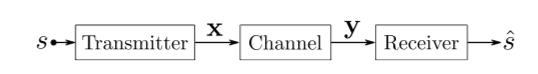
\includegraphics[height= 2cm, width=18cm]{project/images/channel.png}
  \caption{\textbf{Simple Communication Channel Model}}
\end{figure}
The transmitter wants to communicate one out of M possible messages s : M = {1,2,...,M} to the receiver making n discrete uses of the channel. To this end, it applies the transformation f to the message s to generate the transmitted signal x = f(s).The communication rate of this communications system is R = k/n, where k = log2(M). In the sequel, the notation (n,k) means that a communications system sends one out of M = 2k messages (k bits) through n channel uses.\\
From a DL point of view, this simple communications system can be seen as a particular type of autoencoder. Typically, the goal of an autoencoder is to find a low-dimensional representation of its input at some intermediate layer which allows reconstruction at the output with minimal error. In this way, the autoencoder learns to non-linearly compress and reconstruct the input. In our case, the purpose of the autoencoder is different. It seeks to learn representations x of the messages s that are robust with respect to the channel impairments mapping x to y (i.e., noise, fading, distortion, etc.), so that the transmitted message can be recovered with small probability of error. In other words, while most autoencoders remove redundancy from input data for compression, this autoencoder often adds redundancy, learning an intermediate representation robust to channel perturbations. The simple scheme of our autoencoder is shown in fig. 3.2
\vspace{3cm}
\begin{figure}[H]
  \centering
    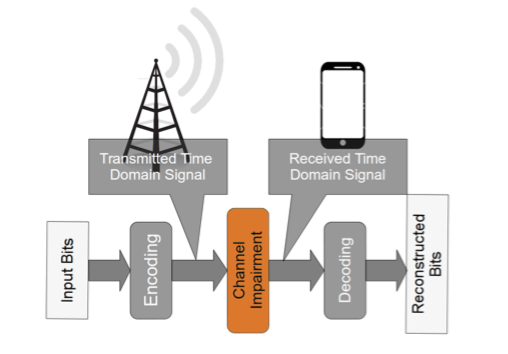
\includegraphics[height= 12cm, width=18cm]{project/images/encoder-decoder.png}
  \caption{\textbf{Modelling the channel as an Autoencoderl}}
\end{figure}

\newpage
\section{Implementation}
We constructed a new gaussian noise layer that adds a random normal noise to the transmitted signal. \\
The network works as is shown if fig. 3.3 and the parameters of the network built are shown in fig. 3.4 where M = 16 and n =128. 

\begin{figure}[H]
  \centering
    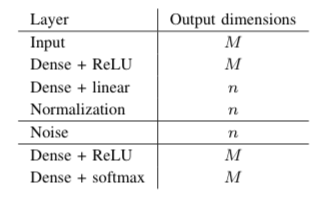
\includegraphics[height= 6cm, width=10cm]{project/images/network.png}
  \caption{\textbf{Autoencoder Network}}
\end{figure}

\begin{figure}[H]
  \centering
    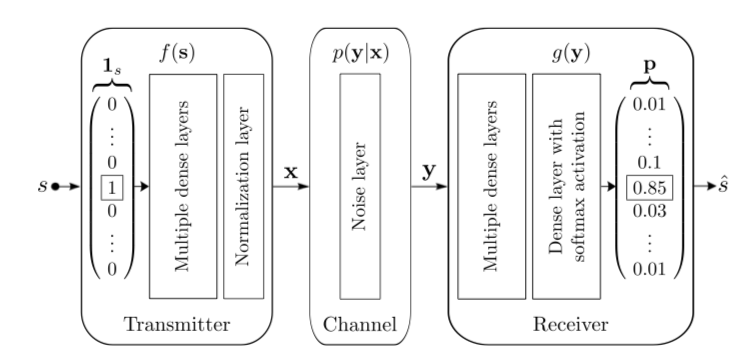
\includegraphics[height= 8cm, width=18cm]{project/images/statisticsOfNetwork.png}
  \caption{\textbf{Network Parameters}}
\end{figure}

\newpage
\section{Problems Faced}
The training was done and tested at a particular SNR but the results were not matching as proposed in the paper. We expected the performance of our autoencoder to match with that of hamming encoder with MLD decoding as shown in the below graph. 

\begin{figure}[H]
  \centering
    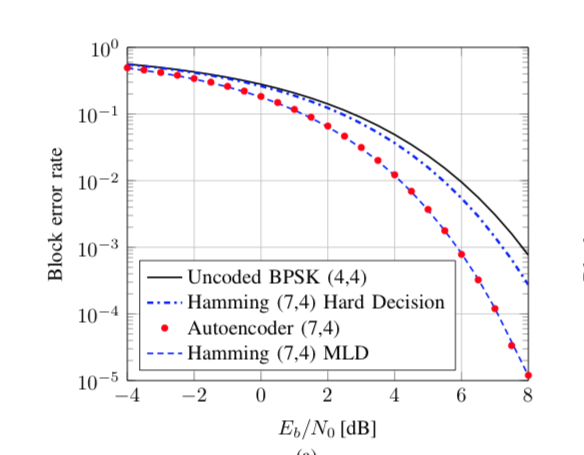
\includegraphics[height= 12cm, width=14cm]{project/images/graph.png}
  \caption{\textbf{Modelling the channel as an Autoencoderl}}
\end{figure}